\documentclass[10pt,a4paper]{report}
\usepackage[utf8]{inputenc}
\usepackage[english]{babel}
\usepackage{amsmath}
\usepackage{amsfonts}
\usepackage{amssymb}
\usepackage{graphicx}
\author{A.M. Ahsan Feroz \\
\texttt{abdullah.feroz@aalto.fi}
\and
Md. Mohsin Ali Khan \\
\texttt{md.m.khan@aalto.fi}
\and
Elena Oat\\
\texttt{elena.oat@aalto.fi}
\and
Hasan M. A. Islam \\
\texttt{hasan.islam@aalto.fi}
\and
Mesbahul Islam Nahin\\
\texttt{mdislam@cs.helsinki.fi} \\
\and
Tutor: Antero Juntunen
}
\title{T-110.5130 Mobile Systems Programming Project Specification}
\begin{document}
\maketitle
\chapter{Introduction}
Smartphones and tablets are ubiquitous everywhere. Typically, a smartphone is a mobile phone built on a mobile operating system, with more advanced computing capability and connectivity than traditional phone. The rapid adoption of mobile platforms is being driven by the numerous applications that allow users to perform everyday transactions. The examples of mobile operating systems (OS) used by modern smartphones are Google's Android, Apple's iOS, Nokia's Symbian, etc. Android is an open-source platform founded in October 2003 by Andy Rubin and backed by Google, along with major hardware and software developers (e.g., Intel, HTC, ARM, Motorola, Samsung). We are very enthusiastic to build application in Android for the course $'$Mobile Systems Programming$'$. The main motivation behind choosing Android platform are the followings:

 \begin{itemize}
   \item Android is the most widely used platform for mobile respecting the number of users and number of applications.
   \item Android app developers use the classic open source Linux OS. Any open source provides help for users to access its source code transparently and is available to any developer who wants to modify it or see how it works.
   \item Google provides all Android developers with an open source software development kit for the Android OS. They can create applications for Android and then test them on an Android simulator before loading them onto an actual Droid phone.
   \item The future of the Android platform looks bright for Android application developers who love to have access to everything. We can expect to see some interesting innovations both from Google and from the public as Android gains popularity.
 \end{itemize}

Nevertheless, our rudimentary plan is to develop a $'$Task Manager$'$ which is initially named as $'$AndroTasker$'$. Now-a-days, people are so busy with their daily activities and hence, it is more likely for one to forget a schedule that might be very important. In the present hi tech world, mobile phones could be a great medium to keep track of the all the things and notify the user in the right time to perform a task. The very first version of our Android Task Manager will be a typical task manager which would be able to maintain and keep track of all of our schedules of every moment. The user can give temporal input to our application and the app will be responsible to remind the user by means of alarm about the temporal events. The reminder can be set for each minutes of a day and in a year. The application will always be running in the background and the reminder will pop up in a small screen at the desired time. The application will also have a view screen which can be used as an widget in the desktop with the list of tasks.




 

\section{Goals and scope}
The primary goal of the project is to learn how to develop a mobile application for Android platform. We want to make sure that all of the group members understand the basic building blocks of an Android Mobile application along with their significance and underlying concepts. We want to make sure that we understand how an Android application interacts with user. And back to back how it interacts with the Android Operating System to get the job done that is requested by the user. We want to learn how to publish an Android application in the market. The secondary goal of the application is to make sure that we understand how to interact with other Android applications. The scope of the project is to develop an application that provides the user functionality to do the following activities:

\begin{description}
 \item 1. View Existing Events
  \begin{itemize}
    \item Day view
    \item Week view
    \item Month view
  \end{itemize}
  
  \item 2. Create New Events
  \item 3. Edit Existing Events
  \item 4. Alarm and Bar notifications of the Events at the due time
\end{description}

\section{Why Andro Task Manager}

The motivation behind choosing the task manager to develop is to learn many aspects of the android development environment, such as

\begin{itemize}
  \item[$\bullet$] How to manage Activity Life Cycle in Android.
  \item[$\bullet$] Building a flexible UI using \texttt{Fragments}
  \item[$\bullet$] design app's screen hierarchy and forms of navigation so that users can effectively and intuitively traverse our app content using various navigation patterns.
  \item[$\bullet$] How to store user and app data (e.g., SQLite)
  \item[$\bullet$] How to interact with other apps (using \texttt{Intent}) i.e., how to exploit Android's one of the most important feature to send the user to another app based on "action" (secondary goal).
\end{itemize}


 Respecting the type of our application, it can be said that this is useful for all range of people who use smart phones smartly and hopefully the number is countless. Task manager can help to manage every aspect of managing task. It reduces the administrative tasks. It will reduce paperwork. It will help to manage resources with greater control.

\chapter{Work practices and tools}

In this chapter, all planned work practices for our project will be outlined in brief such as how our group works, how the documentation of our work will assembled so that each and every member could be able to know the events though one may absent for any particular reason.

\section{Time Tracking}
For tracking our progress and communication, we mostly use Facebook. A private group was created, which includes all the members of our group. FB is our main platform to agree on when/where the next meeting is, as well as share our thoughts and useful links.
\section{Meetings and Documentation}
We meet once a week, as a rule. Meeting duration is for three hours. We have also met once for the whole day, when we were working on the UI of our application. The time we spent is written down and is tracked by the project leader. 

We haven’t had to deal with documentation very much, as we make decisions during the meeting and since every member is present, we are all up to date with the situation. For other cases we use Google Docs. And again, some decisions are made on Facebook group wall and all people who have access could follow up with the process. 

In general, we don’t have a clear division on who will do what, we just have project leader who coordinates the meetings times and does other organizational task.

\section{Version Control}
Git is a free and open source distributed version control system designed to efficiently handle everything from small to very large projects with a good speed. Git is easy to learn and has a tiny footprint with lightning fast performance. It subordinates SCM tools like Subversion, CVS, Perforce, and ClearCase with features like cheap local branching, convenient staging areas, and multiple workflows.

We have decided to use \texttt{Github} for sharing code and other resources and controlling versions. Every group member has an account on \texttt{Github}. A repository was created, which serves as a place for common development. All commits are accompanied by a message which states what changes have been made to the previous version.

\section{Design}

In order to better understanding, we are going to develop custom calender day view, week view and month view. Android development kit provides \texttt{Layout} such as \texttt{Relative Layout}, \texttt{List View}, \texttt{Grid View}, \texttt{Table Layout}. In some UI design, Grid View seems advantageous. We can also use the combination of these making our UI attractive. 

\begin{figure}[h!]
\begin{center}$
\begin{array}{cc}
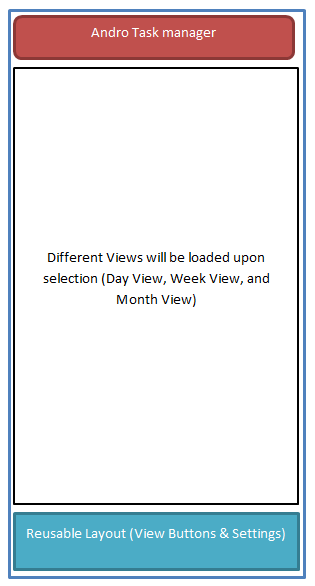
\includegraphics[scale=0.5]{hl.png}  &
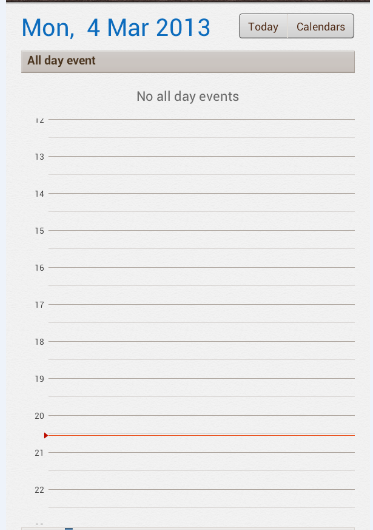
\includegraphics[scale=0.5]{day.png}
\end{array}$
\end{center}
\caption{High level view and Day view}
\label{hd}
\end{figure}

\begin{figure}[h!]
\begin{center}$
\begin{array}{cc}
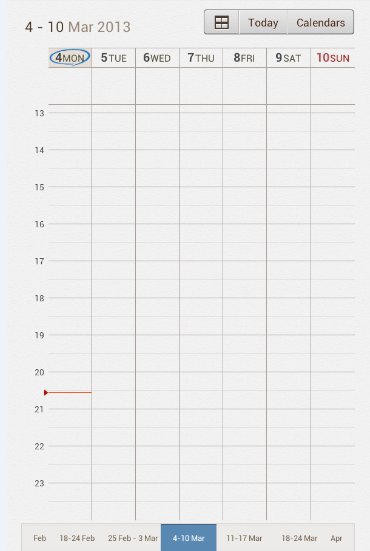
\includegraphics[scale=0.5]{week.png} &
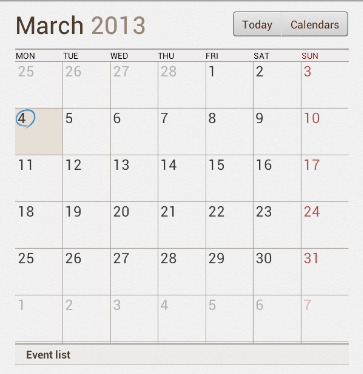
\includegraphics[scale=0.5]{month.png}
\end{array}$
\end{center}
\caption{Week and Month view UI}
\label{wm}
\end{figure}

\begin{figure}[h!]
\begin{center}
	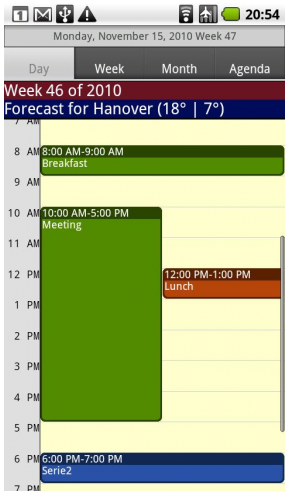
\includegraphics[scale=0.7, trim=125 0 50 0]{dvc.png}
	\caption{Scheduler Sample (Imaginary)}
\end{center}
\label{dvc}
\end{figure}



Figure~\ref{hd} provides the core fundamental UI for our project. Different view will be loaded upon user \texttt{"action"}. At the lower portion, it indicates \texttt{\textbf{Reusable layout}}  of Android feature. Android offers a variety of widgets to provide small and re-usable interactive elements to efficiently reuse complete layouts and embed another layout inside the current layout. Reusing layouts is particularly powerful as it allows you create reusable complex layouts that is expected for our desired project. It also will provide help for our application to extract commonalities across multiple layouts, managed separately. 

We ideate the week view and month view as like Figure~\ref{wm}. User can store their task in our app. Android provides several options to save persistent application data. As app data should be \texttt{private}, we can utilize \texttt{Shared Preferences} and \texttt{SQLite Storage}. Our app should not require that much storage. Figure~\ref{hd} represents an imaginary figure with user's stored tasks. UI will use \texttt{GridView}  or\texttt{Listview} displaying items in a two-dimensional, scrollable grid. The grid items are automatically inserted to the layout using a \texttt{ListAdapter}.

For testing purposes we use our own devices (Android smartphones), as this provides an easier and faster way to check the latest changes.

\section{Quality Assurance}

We try to only follow the official tutorials and documentation that is provided by developer.android.com and avoid amateur blogs. However, this is sometimes challenging, because not all answers are available on official Android’s website. YouTube channels help also in learning basics, e.g. Marakana’s channel. We try to also read the best practices that were set by Android community, but sometimes it is hard to do it in the beginning, because you don’t know yet all the concepts.

\section{Tools}
Tools that will be used for this project are the followings: 
\begin{itemize}
\item[i.] Android devices (Android 2.3.5, Android 4.0, Android 4.1.2)
\item[ii.] Eclipse for Mobile Developers (Version: Juno Service Release 1)  + ADT
\item[iii.] GIT, Github application on Windows
\item[iv.] Google docs             	
\item[v.] Facebook group. 

\end{itemize}
\pagebreak

\section{Schedule and resources}

\begin{center}
\begin{table}[h]\footnotesize
  \begin{tabular}{| p{5cm}  | p{2cm} | p{2cm} | p{2cm} |}
  

    \hline
    \textbf{Task}  & \textbf{Deadline} & \textbf{Required Hours} & \textbf{Load Distribution per person} \\ \hline
    Finalizing The Application to be developed & 25-Jan-13  & 10 &2\\ \hline
    Finalizing the Scope of the Application& 31-Jan-13 &10  &2 \\ \hline
    Finalizing the User Interface, Data Flow and Browsing Sequence	& 10-Feb-13 & 30 &6\\ \hline
    Environment Setup for Coding &15-Feb-13  & 25 &5 \\ \hline
    Understanding the Basic Building Blocks of an Android Application and Developing a Test Application &25-Feb-13 &25 &5\\ \hline
    Developing the Designed User, Interface &15-Mar-13  &50  &10 \\ \hline
    Developing the Underlying Events, Implement the Data Flow and Browsing Sequence &15-Apr-13  & 150  &30\\ \hline
    Preparing Test Case of the Application & 20-Apr-13 & 25 & 5 \\ \hline
    Testing1 & 25-Apr-13 & 25&5 \\ \hline
    Bug Fixing 1& 27-Apr-13 &40   &8  \\ \hline
    Testing2 & 30-Apr-13  & 25 &5  \\ \hline
    Bug Fixing 2 & 5-May-13   &40   &5 \\ \hline
      
  \end{tabular}
   \caption{Scheduling and Load Distribution.}
    \label{comparison}  
  \end{table}
\end{center}
\chapter{System overview}
To create, edit (Update or Delete) or view an event an user first select a suitable view: day, week or month view. If user choose day view then a listview with hours of the selected day will be shown. User can select a time slot to create new event or edit existing event.

\begin{figure}[h!]
\begin{center}
	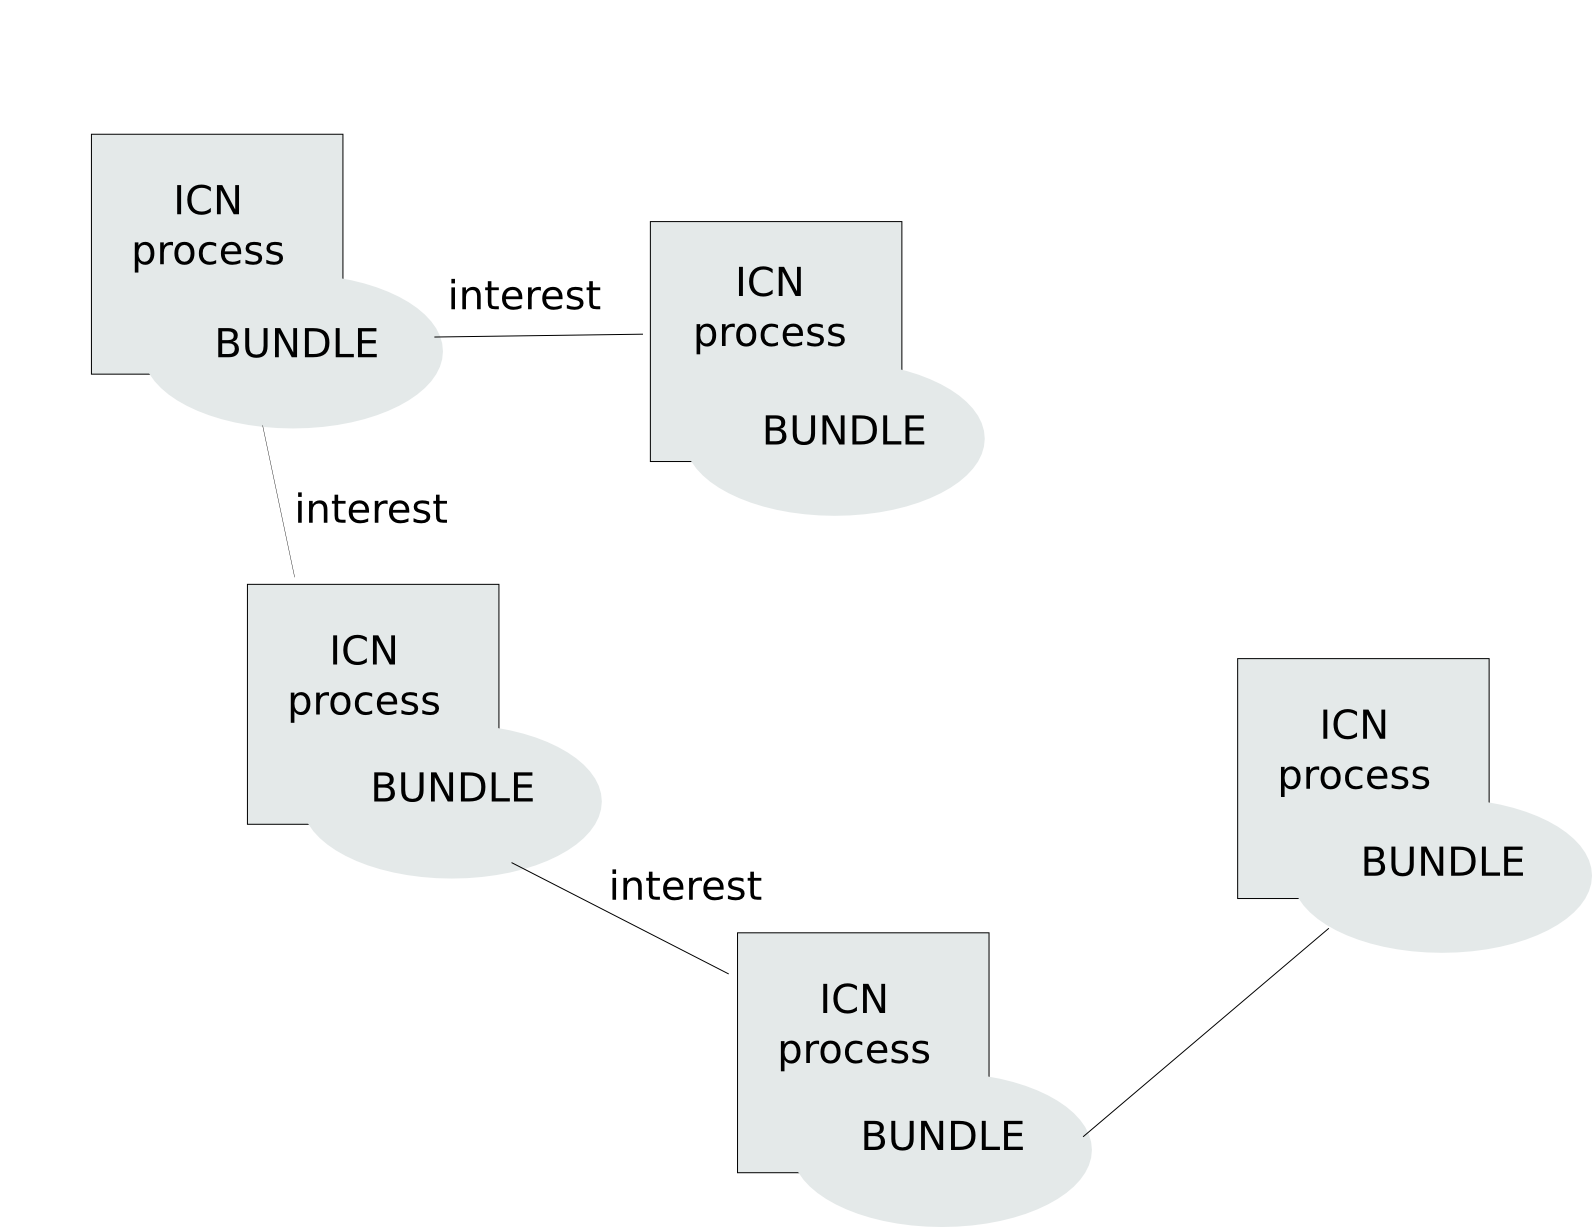
\includegraphics[scale=0.25, trim=125 0 50 0]{path4019.png}
	\caption{Basic System Overview}
\end{center}
\end{figure}

User will be notified based on the stored tasks into our app's database. 
\section{Requirements}
Functional requirements states what the system can do. Some functional requirements are as follows:
\begin{description}
\item[Functional Requirements]: \\

\begin{description}
 \item[1. Display:] AndroTask Manager will pose the following views for users.  
   \begin{itemize}
     \item Day view
     \item Week view
     \item Month view 
     \end{itemize}
 \item[2. Users Action:] An user can do the following actions:  
   \begin{itemize}
     \item Create Event
     \item Edit Event
     \item View Event
     \item Delete Event    
   \end{itemize}
  \item[3. Notification] There will be notification prior to an event.  
   \begin{itemize}
     \item alarm notification
     \item visual notification on mobile screen
   \end{itemize}
  \item[4.Settings:] Users can set options according to their preference:
    \begin{itemize}
     \item User can set alarm type and sound
     \item User can set weekdays and weekends
   \end{itemize}
  \item[5. onStart] Application will starts with Day View of current date.
  \item[6. Default] If there are existing event(s) of current date then the event(s) will load and show by default
 \end{description}
 \item[Non-Functional Requirements:] qualities of the system.
   \begin{itemize}
     \item A user can’t create an event for a day that has passed away already
     \item The design is user friendly
   \end{itemize}
 
 
\end{description}
\end{document}
